
\chapter{Introduction}
\label{ch:INTR}
\section{Introduction}
The HUMAN population is continually expanding, as is the demand for food. According to
UN projections[1,] the human population will reach 9.7 billion in 2050, up from the present
estimate of 7.2 billion. Given that the majority of population growth (about 80% in the next
30 years) occurs in least developed nations, where food shortage is a major issue, reducing
food waste in these countries should be a primary goal. Global yield losses are projected to
range from 20% to 40% [2], with many farmers losing their whole crop. Traditional disease
detection methods necessitate hand inspection of plants by professionals. This method must
be continuing and pricey for large farms, or it may be utterly out of reach for many small
farmers in rural areas. As a result, in recent decades, many initiatives to automate sickness
detection have been made. Hyperspectral images are one of the most effective methods.
Hyperspectral images are used to monitor broad areas and are often captured by satellite or
aerial imaging equipment. This technique has several drawbacks, including a high cost of
equipment, high dimensionality, and a small number of samples, all of which make it
unsuitable for machine learning analysis (ML). Because of recent advances in computer
vision and the availability of affordable hardware, RGB image analytics are currently the
most often utilised technique. Another reason to look at RGB photos is that, because to the
widespread usage of cellphones, these solutions can reach even the most remote locations.
Traditional machine learning (ML) methodologies or the deep learning (DL) method can be
used to analyse RGB photos. Image pre-processing and attribute extraction are used in
traditional methods, which are then fed into one of the machine learning algorithms. Support
vector machines (SVM), k-nearest neighbours (k-NN) and full connected neural networks
(FCNN), decision trees, and random forests are all popular techniques. For image
classification problems, researchers have turned nearly totally to DL techniques in recent
years. Classic approaches almost always outperform when a small dataset is provided, and
they can be used without the usage of hand-made features. In this study, we compare the DL
approach to established ML algorithms for plant disease categorization.
\begin{definition}
vvhffff
\end{definition}

\begin{figure}[bpht]
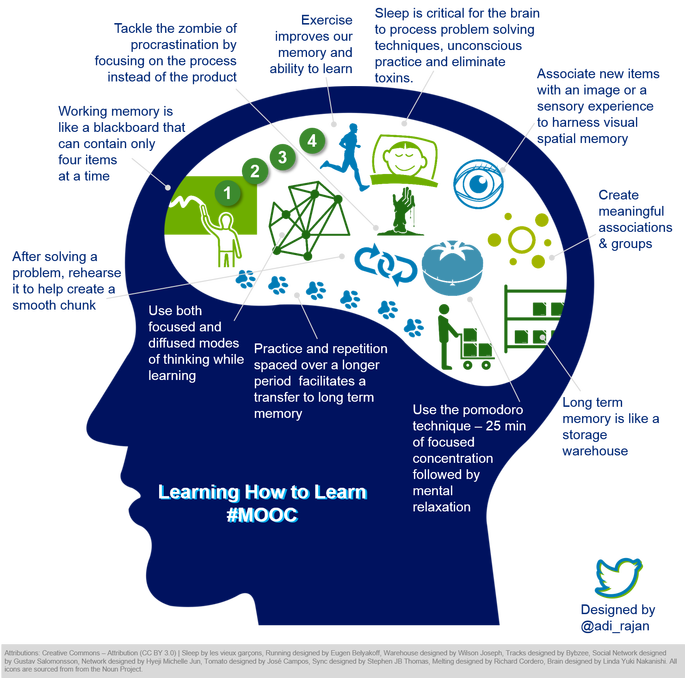
\includegraphics{Chapter1/LHTL}
\caption{Learning how to learn}
\end{figure}

\section{Motivation}
Shortcomings in the previous work / referenced paper,  Brief importance of the work in the present context,  Significance of the possible end result etc.

\section{Objectives}

\section{Organization of Report}

Organization of the project report (chapter wise)





